\documentclass[12pt,a4paper,italian]{article}


\usepackage[italian]{babel}
\usepackage[latin1]{inputenc}
\usepackage{amsmath}
\usepackage{amsfonts}
\usepackage{amssymb}
\usepackage{color}
\usepackage{xcolor}
\usepackage{hyperref}
\usepackage[all]{hypcap}
\usepackage{ifthen}
\usepackage{wrapfig}
%\author{Piero Bizzotto}
\usepackage[top=2cm,bottom=5cm,left=80pt,right=80pt]{geometry}
\usepackage{graphicx}
\DeclareGraphicsExtensions{.jpg,.png}

\newcommand{\ajax}{AJAXDRAW}
\newcommand{\sito}{\href{http://ajaxdraw.sourceforge.net}{http://ajaxdraw.sourceforge.net}}

\setlength{\parindent}{0pt} %settato indentazione di default 
\setlength{\headheight}{3cm} %settato grandezza header...in altre parole, quanto distanzio il doc dall'intestazione

\usepackage{fancyhdr} %pacchetto per le intestazioni
\pagestyle{fancy} %uso del pacchetto


\fancyhead{} %annulla head di default
\fancyfoot{} %annulla foot di default


\usepackage{lastpage} %setto pg di pgtot a rfoot
     \rfoot{pagina \thepage\ di \pageref{LastPage}}


\lfoot{Versione: \insertversion} %setto versione doc a lfoot
\renewcommand{\footrulewidth}{0.5pt} %ridefinisco il valore della riga di intestazione
\renewcommand{\headrulewidth}{0.5pt} %ridefinisco il valore della riga di pie' di pagina

\newcommand{\insertversion}{0.0} %definisco il nuovo comando per inserire la versione


\lhead{  \begin{Huge} \ajax \end{Huge} \\  %intestazione di sinistra
					%\begin{Large}	Software per il Disegno Grafico\\ in Tecnologie Web \end{Large}  
					\begin{normalsize}\sito \end{normalsize}
			%\\ versione documento: \insertversion\ del \today} %setto l'intestazione sx
		}
\rhead{ %includo logo nell'intestazione dx
	 	
\includegraphics[scale=0.5]{../logo/logo.png}  
}


%CREAZIONE ELENCHI NUMERATI PERSONALIZZATI
\newcounter{Lcount}
\newcounter{Rcount}
\setcounter{Lcount}{0}
\setcounter{Rcount}{0}

\newenvironment{elenconumerato}[2][ ]
{
  \begin{list}{#1\arabic{Lcount}.}
    {
	\setcounter{Rcount}{\value{Lcount}}
	\setcounter{Lcount}{0} 
	\usecounter{Lcount} 
\addtolength{\leftmargin}{#2pt}
	}
}
{
  \end{list}
 \setcounter{Lcount}{\value{Rcount}}
}

%CREAZIONE ELENCHI PUNTATI
\newenvironment{elencopuntato}[1][]
{
\begin{list}{\textbullet} %\itemindent=#1pt
	{
	\addtolength{\leftmargin}{#1pt}
	}
} 
{
\end{list}
}


\newenvironment{elencodescrittivo}[1][]{\begin{description} \setlength{\itemindent}{#1pt} \addtolength{\leftmargin}{#1pt}} {\end{description}}

\newcommand{\TITOLODOC}{Titolo}

%footer centrale
\cfoot{ \TITOLODOC \\  E-mail:    \href{ mailto:webshape.contact@gmail.com}{ webshape.contact@gmail.com}  }

%INSERIMENTO IMMAGINI
\newcommand{\imagerealsize}[1]{\vspace{20pt} \includegraphics{#1} }
\newcommand{\imageadapted}[1]{\vspace{20pt} \includegraphics[width=1\textwidth]{#1} }

\newcommand{\glosspath}{.\glossario}
\newcommand{\gloss}[1]{\hyperref{\glosspath~\glossario.pdf}{}{#1}{#1}}

\hypersetup{
    %bookmarks=true,         % show bookmarks bar?
    %unicode=false,          % non-Latin characters in Acrobat’s bookmarks
	%pdftoolbar=true,        % show Acrobat’s toolbar?
	%pdfmenubar=true,        % show Acrobat’s menu?
    %pdffitwindow=true,      % page fit to window when opened
    %pdftitle={My title},    % title
    %pdfauthor={Author},     % author
    %pdfsubject={Subject},   % subject of the document
    %pdfnewwindow=true,      % links in new window
    %pdfkeywords={keywords}, % list of keywords
    colorlinks=true,         % false: boxed links; true: colored links
    linkcolor=black,           % color of internal links
    %citecolor=green,        % color of links to bibliography
    %filecolor=magenta,      % color of file links
    urlcolor=teal    % color of external links
%	linktocpage=false;
}


%COLORAZIONE TESTO
\newcommand{\blue}[1]{{\color {blue} #1}} 
\newcommand{\red}[1]{{\color {red} #1}}
\newcommand{\green}[1]{{\color {green} #1}}
\newcommand{\sezione}[1]{\leftskip=0pt \section{#1} \leftskip=18pt}
\newcommand{\subsezione}[1]{\leftskip=18pt \subsection{#1} \leftskip=36pt}
\newcommand{\subsubsezione}[1]{\leftskip=36pt \subsubsection{#1} \leftskip=54pt}
\newcommand{\subsubsecindent}{54}
\newcommand{\subsecindent}{36}
\newcommand{\secindent}{18}
\newcommand{\normindent}{8}
\newcommand{\code}[1]{{\bfseries \texttt{#1}}}
\newcommand{\paragrafo}[1]{\leftskip=36pt \paragraph{#1} \leftskip=54pt}
\newcommand{\subparagrafo}[1]{\leftskip=54pt \subparagraph{#1} \leftskip=72pt} %BASE!!!
\usepackage{multirow}
 
\title{\TITOLODOC}
\author{Carollo Mirko}
 
\begin{document}
 
\renewcommand{\insertversion}{4.0} %INSERIRE LA VERSIONE QUI DENTRO STILE x.x.xx
\renewcommand{\TITOLODOC}{Piano di qualifica} %INSERIRE IL TITOLO DEL DOCUMENTO DA FAR COMPARIRE A PIE PAGINA
\renewcommand{\glosspath}{.\glossario} %INSERIRE PERCORSO RELATIVO
 
%%%%%%%%%%%%%%%%%%%%%%PARTE DA NON MODIFICARE%%%%%%%%%%%%%%%%%
\begin{titlepage}
\begin{center}
  \begin{Large}  \today \end{Large}
\end{center}
 
\vspace{20pt}
 
\begin{center}
  \begin{Huge}
        \textbf{\ajax}
  \end{Huge}
\end{center}      
 
\begin{center}
  \begin{large}
        \textbf{Software per il Disegno Grafico\\ in Tecnologie Web}
  \end{large}
\end{center}      
 
\vspace{20pt}
 
\begin{center}

\includegraphics[width=150pt]{../logo/logo}
\end{center}
 
\vspace{170pt}
\begin{center} %INSERIRE ALL'INTERNO IL TITOLO DOCUMENTO CHE COMPARIRA NELLA PAGINA INIZIALE        
  \begin{Huge}
        \textbf{\TITOLODOC}
  \end{Huge}
      \\
\end{center}
\vspace{190pt}
\begin{center}
Versione: \insertversion
\end{center}
\end{titlepage}
 
\newpage
%%%%%%%%%%%%%%%%%%%%%%FINE PARTE DA NON MODIFICARE%%%%%%%%%%%%%%%%%
 
\begin{center} %INSERIRE ALL'INTERNO IL TITOLO DOCUMENTO CHE COMPARIRA NELLA PAGINA INIZIALE
  \begin{Huge}  
        \textbf{\TITOLODOC}
      \\
  \end{Huge}
\end{center}
 
%\setlength{\parindent}{18pt} %settato indentazione di default
\section*{\LARGE Sommario:} %SEZIONE SOMMARIO
\indent \indent
Il presente documento descrive le strategie per la verifica della correttezza dei documenti e del codice prodotto, adottate dall'azienda WebShape, e comprende un resoconto delle relative attivit\`a effettivamente svolte.
 
\section*{\LARGE Stato del documento:}
\indent \indent
  Formale Esterno
 
\section*{\LARGE Redazione:}
  \begin{table}[!h]
    \begin{center}
      \begin{tabular}
        {|c|c|}
        \hline
        %%%%%%%%%%%%%%INTESTAZIONE COLONNE%%%%%%%%%%%%%%%%%%%%%%%%%%%%%%%%
        \multicolumn{2}{|c|}{ \textbf{Redazione} } \\
        \hline
        \textbf{Fase} & \textbf{Redattori} \\
        %%%%%%%%%%%%%%FINE INTESTAZIONE COLONNE%%%%%%%%%%%%%%%%%%%%%%%%%%%%%%%%%%%%%%
        \hline
        %%%%%%%%%%% PARTE DA MODIFICARE %%%%%%%%%%%%%%%%%%%%%%%%%%%%%%%%%%%%%%%%%%    
        Pre-RR & Dissegna Stefano\\
        \hline
        RR-RPP & Carollo Mirko\\
        
        \hline
        \multirow{2}{*}{RPP-RQ} & Carollo Mirko \\
							& Dissegna Stefano \\
        
        \hline
        \multirow{1}{*}{RQ-RA} & Dissegna Stefano \\
        \hline

        %%%%%%%%%%% FINE PARTE DA MODIFICARE %%%%%%%%%%%%%%%%%%%%%%%%%%%
      \end{tabular}
      \caption{Lista Redattori} %INSERIRE DIDASCALIA - SE NECESSARIA -
      \label{tabredazione}
    \end{center}
  \end{table}  
 
\section*{\LARGE Verifica:}
\begin{table}[!h]
  \begin{center}
    \begin{tabular}
      {|c|c|}
      \hline
      %%%%%INTESTAZIONE COLONNE%%%%%%%%%%%%%%%%%%%%%%%%%%%%%%%
      \multicolumn{2}{|c|}{ \textbf{Verifica} } \\
      \hline
      \textbf{Fase} & \textbf{Verificatori} \\
      %%%%%%%%%%%%%%FINE INTESTAZIONE COLONNE%%%%%%%%%%%%%%%%%%%%%%%%%%%%%%
      \hline
      %%%%%%%%%%% PARTE DA MODIFICARE %%%%%%%%%%%%%%%%%%%%%%%%%%%%%%%%%%%%%%    
      Pre-RR & Dal Bosco Davide\\
                 
      \hline
      RR-RPP & Geremia Mirco \\
                  
      \hline
      RPP-RQ & Bizzotto Piero \\
                  
      \hline
      RQ-RA & Rizzo Maurizio \\
                  
      \hline
      %%%%%%%%%%% FINE PARTE DA MODIFICARE %%%%%%%%%%%%%%%%%%%%%%%%%%%%%%%%%%%
    \end{tabular}
    \caption{Lista Verificatori} %INSERIRE DIDASCALIA - SE NECESSARIA -
    \label{tabverifica}
  \end{center}
\end{table}
 
 
\section*{\LARGE Approvazione:}
\begin{table}[!h]
  \begin{center}
    \begin{tabular}
      {|c|c|}
      \hline
      %%%%%INTESTAZIONE COLONNE%%%%%%%%%%%%%%%%%%%%%%%%%%%%%%%
      \multicolumn{2}{|c|}{ \textbf{Approvazione} } \\
      \hline
      \textbf{Fase} & \textbf{Approvatori} \\
      %%%%%%%%%%%%%%FINE INTESTAZIONE COLONNE%%%%%%%%%%%%%%%%%%%%%%%%%%%%%%
      \hline
      %%%%%%%%%%% PARTE DA MODIFICARE %%%%%%%%%%%%%%%%%%%%%%%%%%%%%%%%%%%%%%    
      Pre-RR & Cunico Marco\\
                 
      \hline
      RR-RPP & Bizzotto Piero \\
                  
      \hline
      RPP-RQ & Dal Bosco Davide \\
                  
      \hline
      RQ-RA & Geremia Mirco \\
                  
      \hline

      %%%%%%%%%%% FINE PARTE DA MODIFICARE %%%%%%%%%%%%%%%%%%%%%%%%%%%%%%%%%%%
    \end{tabular}
    \caption{Lista Approvatori} %INSERIRE DIDASCALIA - SE NECESSARIA -
    \label{tabapprovazione}
  \end{center}
\end{table} 
 
\section*{\LARGE Lista di Distribuzione:}
 
  \begin{elenconumerato}{\normindent}
    \item WebShape
    \item I committenti Conte Renato e Vardanega Tullio in rappresentanza \\ dell'azienda proponente Zucchetti SPA
  \end{elenconumerato}
 
\newpage
 
 
 
\section*{\LARGE Registro delle Modifiche:}
 
 
\begin{center}
  \begin{table}[h]
     \begin{tabular*}
      {1\textwidth}%
        {@{\extracolsep{\fill}}|p{0.1\textwidth}|p{0.54\textwidth}|p{0.26\textwidth}|}
       \hline
%%%%%%%%%%%%%%INTESTAZIONE COLONNE%%%%%%%%%%%%%%%%%%%%%%%%%%%%%%%%%%%%%%%%%%%%%%%%%%%%%%%%%%%%%%
      \textbf{Versione} & \textbf{Descrizione} & \textbf{Autore} \\
%%%%%%%%%%%%%%FINE INTESTAZIONE COLONNE%%%%%%%%%%%%%%%%%%%%%%%%%%%%%%%%%%%%%%%%%%%%%%%%%%%%%%%%%%%%%%
     \hline
%%%%%%%%%%% PARTE DA MODIFICARE %%%%%%%%%%%%%%%%%%%%%%%%%%%%%%%%%%%%%%%%%%%%%%%%%%%%%%%%%%%%%%%%%
     4.0 &   22$\slash$03$\slash$2009 Modifiche per rilascio RQ & Dissegna Stefano\\
      \hline
     3.6 &    19$\slash$03$\slash$2009 Aggiunta sezione sulle azioni da intraprendere dopo un errore & Dissegna Stefano\\
      \hline
     3.5 &    18$\slash$03$\slash$2009 Breve descrizione dei test manuali & Dissegna Stefano\\
      \hline
     3.4 &    18$\slash$03$\slash$2009 Descrizione dei test automatici & Dissegna Stefano\\
      \hline
     3.3 &    18$\slash$03$\slash$2009 Resoconto dei test & Dissegna Stefano\\
      \hline
     3.2 & 18$\slash$03$\slash$2009 Giustificato meglio la copertura attesa & Dissegna Stefano\\
      \hline
     3.1 &    18$\slash$03$\slash$2009 Correzioni minori & Dissegna Stefano\\
      \hline
     3.0 &    7$\slash$03$\slash$2009 Sistemazione in vista rilascio RQ & Carollo Mirko\\
      \hline
      2.2 &  6$\slash$03$\slash$2009 Valutazione qualit\`a prima di consegna RQ & Dissegna Stefano \\
      \hline
      2.1 &  5$\slash$03$\slash$2009 Aggiunte metriche di valutazione ed aspettative & Dissegna Stefano \\
      \hline     2.0 &    23$\slash$01$\slash$2009 Verifica finale in preparazione al rilascio per la RPP & Carollo Mirko\\
      \hline 
      1.1 &    19$\slash$01$\slash$2009 Aggiunti strumenti e procedure di automazione & Carollo Mirko\\
      \hline
      1.0 &    09$\slash$12$\slash$2008 Verifica finale in preparazione al rilascio & Dissegna Stefano\\
      \hline
             0.3 & 7/12/2008 Correzioni in seguito a revisione & Dissegna Stefano \\
       \hline
            0.2 & 7/12/2008 Impaginazione e modifiche minori & Dissegna Stefano \\
       \hline
            0.1 & 23/11/2008 Piano di qualifica per la progettazione & Dissegna Stefano \\
            \hline
            0.0 & 22/11/2008 Bozza iniziale & Dissegna Stefano \\
             \hline
%%%%%%%%%%% FINE PARTE DA MODIFICARE %%%%%%%%%%%%%%%%%%%%%%%%%%%%%%%%%%%%%%%%%%%%%%%%%%%%%%%%%%%
    \end{tabular*}
  \caption{tabella delle modifiche} %INSERIRE DIDASCALIA - SE NECESSARIA -
  \label{tab:modifiche}
  \end{table}
\end{center}
 
 
\newpage
\thispagestyle{fancy}
\tableofcontents
\thispagestyle{fancy}
\newpage
 
\sezione{Introduzione}
 
\subsezione{Scopo del documento}
Il presente documento definisce il livello di qualit\`a atteso del prodotto e del processo di realizzazione dello stesso, oltre che l'aderenza del prodotto stesso a quanto descritto nel documento \textit{AnalisiDeiRequisiti} (versione 3.0), indica le metodologie da adottare per assicurare la qualit\`a e riporta le attivit\`a svolte inerenti la gestione della qualit\`a.
 
\subsezione{Scopo del prodotto}
Il prodotto intende permettere la realizzazione di grafica vettoriale tramite una comoda interfaccia web.
 
\subsezione{Glossario}
Si veda il \textit{Glossario}.
 
\subsezione{Riferimenti normativi}
Il presente documento \`e redatto in accordo con le norme interne di WebShape, raccolte nel documento \textit{NormeDiProgetto} (versione 3.0) consegnato assieme a questo documento, e consultabile inoltre dal repository pubblico al quale WebShape si appoggia per i suoi progetti.
 
\sezione{Visione generale della strategia di verifica}
 
\subsezione{Organizzazione, pianificazione strategica e temporale, responsabilit\`a}
Le attivit\`a di verifica si dovranno svolgere immediatamente in seguito ad una modifica, o ad un insieme di modifiche. Qualora non sia possibile svolgere l'attivit\`a in modo automatico, onde evitare di attivare un'intero ciclo di verifica con gli annessi costi per delle modifiche di scarso rilievo, l'attivit\`a sar\`a svolta quando le differenze tra la versione attuale del prodotto e la versione su cui \`e stata applicata l'ultima verifica sono sufficientemente rilevanti. \`E compito di chi effettua le modifiche di segnalare ai verificatori la necessit\`a di un'attivit\`a di verifica. Il responsabile della qualifica dovr\`a accertarsi che il tutto si svolga correttamente e che segua quanto descritto nel presente documento.
\paragraph{Verifica dei documenti} Il revisore, attraverso un'attenta lettura del documento, deve controllare, in ordine crescente di importanza, che:
\begin{elenconumerato}[\textbf{}]{\subsubsecindent}
\item la grammatica e la sintassi siano corrette
\item la formattazione del documento sia corretta e segua gli standard contenuti nelle \textit{NormeDiProgetto}
\item i concetti vengano espressi in modo chiaro e non ambiguo
\item i concetti espressi siano corretti
\item il documento sia completo
\item il documento risolva il problema corretto
\end{elenconumerato}
\paragraph{Verifica del progetto architetturale}
Il progetto architetturale dovr\`a essere controllato secondo le seguenti caratteristiche:
\begin{elenconumerato}[\textbf{}]{\subsubsecindent}
\item Aderenza alle \textit{NormeDiProgetto}.
\item Completezza: per controllare l'aderenza ai requisiti, dovr\`a essere verificata la tracciabilit\`a tra ogni requisito e la parte, o le parti, che lo soddisfano nel progetto.
\item Sufficienza: ogni elemento del progetto dovr\`a, o soddisfare un requisito, o essere una dipendenza, diretta o indiretta, di un elemento necessario a soddisfare un requisito, in modo che nessuna parte del progetto risulti superflua.
\item Estendibilit\`a e manutenibilit\`a: il progetto dovr\`a prevedere la possibilit\`a che il prodotto possa essere facilmente esteso e mantenuto in futuro.
\item Scalabilit\`a: considerata la necessit\`a da parte dell'applicazione di un server, la fase di progettazione dovr\`a assicurare che il server sia in grado di gestire un numero elevato di client contemporaneamente senza che l'utente noti problemi di performance.
\end{elenconumerato}
\paragraph{Verifica del progetto di dettaglio}
Il progetto di dettaglio dovr\`a soddisfare i seguenti aspetti:
\begin{elenconumerato}[\textbf{}]{\subsubsecindent}
\item Aderenza alle \textit{NormeDiProgetto}.
\item Completezza: ogni elemento presente nel progetto architetturale dovr\`a essere presente anche nel progetto di dettaglio. Non dovranno inoltre essere presenti delle lacune tra un elemento del progetto e la sua effettiva realizzazione.
\item Sufficienza: non dovranno essere presenti elementi non strettamente necessari alla realizzazione del progetto architetturale.
\item Applicabilit\`a: il progetto dovr\`a essere realizzabile dai programmatori usando le tecnologie previste.
\end{elenconumerato}
\paragraph{Verifica del codice}
La verifica del codice si compone dei seguenti aspetti:
\begin{elenconumerato}[\textbf{}]{\subsubsecindent}
\item Verifica automatica: verr\`a effettuata tramite test di unit\`a predisposti dai verificatori. I test dovranno coprire tutto il codice, a eccezione delle parti il cui funzionamento dipende da input esterni non simulabili in un test di unit\`a, come ad esempio il codice che gestisce gli eventi generati dal movimento del mouse, oppure da effetti secondari i cui risultati non siano facilmente confrontabili in modo automatico, ad esempio come appare l'aspetto grafico del programma sullo schermo dell'utente. I test dovranno accertare il corretto funzionamento delle unit\`a di codice anche con input limite. Per effettuare i test di unit\`a ci si avvarr\`a del software \textit{QUnit}. Per controllare che i test coprano il codice nella sua interezza (salvo le eccezioni gi\`a descritte) si utilizzer\`a \textit{JSCoverage} per controllare quali linee non vengono eseguite durante i test di unit\`a. Una pi\`u dettagliata descrizione di questi strumenti \`e disponibile nelle \textit{NormeDiProgetto}.
\item Prova del prodotto: sar\`a effettuata eseguendo l'applicazione e interagendo con essa, assicurandosi che corrisponda a quanto progettato.
\item Confronto con altri software gi\`a esistenti: requisito fondamentale del prodotto \`e la capacit\`a di generare immagini in formato \underline{SVG}. Per assicurarsi che i file generati siano corretti, si caricheranno su software la cui correttezza \`e nota (ad esempio \textit{Inkscape}) e ci si assicurer\`a che le immagini visualizzate corrispondano con quanto disegnato dall'utente.
\item Analisi statica del codice per controllare che le norme di codifica siano rispettate ed alla ricerca degli errori pi\`u comuni. L'editor JavaScript utilizzato, \textit{emacs} con \textit{js2-mode}, permette di catturare la maggior parte di questi errori mentre il codice viene digitato, mentre altri errori verranno ricercati tramite il programma \textit{JSLint}.
\item Analisi del codice tramite \textit{walkthrough}, alla ricerca di eventuali errori. Questa modalit\`a di verifica  verr\`a applicata su tutto il codice al termine di ogni iterazione.
\end{elenconumerato}
 
 
\subsezione{Risorse necessarie, risorse disponibili}
\paragraph{Documenti} Ogni documento sar\`a verificato da un revisore. Sarebbe auspicabile che a documenti particolarmente importanti, come ad esempio la definizione di prodotto, venissero assegnati due revisori, ma i costi eccessivi associati a una tale scelta non lo permettono.
\paragraph{Codice} Il numero di verificatori da assegnare ad un dato modulo di codice varieranno in base alle esigenze del modulo stesso.
 
\subsezione{Strumenti, tecniche, metodi}
Per il tracciamento degli errori e delle loro soluzioni ci si avvarr\`a degli strumenti di bug tracking messi a disposizione da \textit{SourceForge} e dagli strumenti di versionamento in uso. Per il debug del codice Javascript direttamente da browser si utilizzer\`a Firebug, un'estensione di Firefox. Le discussioni tra i verificatori e gli autori delle modifiche avverrano tramite il sistema di commenti di \textit{GitHub} qualora si tratti di annotazioni di scarsa entit\`a, mentre discussioni pi\`u rilevanti avverranno nel gruppo di discussione interno all'azienda. Entrambi i sistemi mantengono in modo persistente le informazioni, permettendo dei riferimenti futuri alle stesse. I verificatori saranno avvisati della necessit\`a di un'attivit\`a di verifica tramite un messaggio nel gruppo di discussione interno.


\subsezione{Infrastrutture e procedure di automazione} 
\begin{figure}[!ht]
\centering
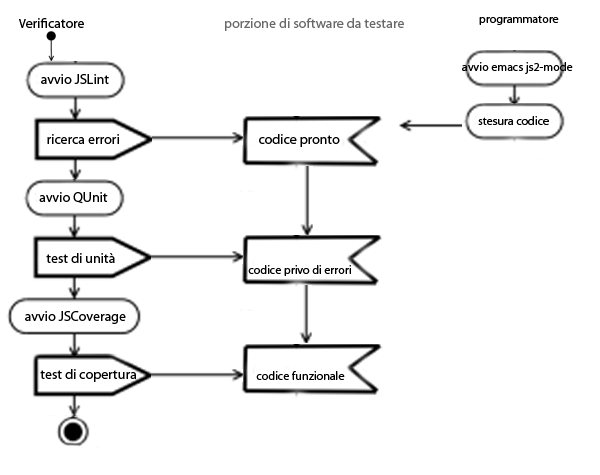
\includegraphics[scale=0.5]{flussi.png}
\caption{flussi}
\end{figure} 
Hanno lo scopo di accelerare tutte le attivit\`a di verifica e impedire errori umani.
Tali attivit\`a potranno quindi essere svolte dopo ogni singolo cambiamento, anche di piccola entit\`a. Saranno predisposte dai verificatori.
Sono raggruppabili in 3 categorie:

\begin{elenconumerato}[\textbf{}]{\subsubsecindent}
\item \textit{Test di unit\`a}
: realizzati tramite il software QUnit. Ogni test ha l'obiettivo di considerare una unit\`a del software per testare se  funziona come dovrebbe. Il verificatore o chiunque altro esegua questo test dovr\`a constatare che il comportamento della porzione di software testato rispetti tutti i vincoli dell'Analisi dei Requisiti. \`E necessario prestare attenzione in quanto superficialit\`a e distrazione umana possono rendere inefficaci e inutili questi test.
\item \textit{Test di copertura}
: realizzati tramite il software JSCoverage. Verificano che i test di Unit\`a siano stati effettuati sull'intera porzione di software stabilita. Hanno l'obiettivo di testare se sono state saltate righe di codice. Utile per garantire l'efficacia dei test di Unit\`a. 
Il verificatore o chiunque altro esegui questo test dovr\`a constatare che tutte le righe di codice siano state coperte nel precedente test di unit\`a, altrimenti sar\`a necessario ripetere e riutilizzare il software QUnit.

\end{elenconumerato}

\subsezione{Metriche di automazione}
Per determinare il numero di test da effettuare su una porzione di software da testare verr\`a considerata la \textit{complessit\`a ciclomatica} di tale pezzo di codice, ossia la metrica strutturale relativa al flusso di controllo. L'azienda ritiene che tale metrica descriva in maniera abbastanza precisa lo sforzo impiegato per realizzare e comprendere una porzione di software. E' compito del verificatore utilizzare tale metrica e stimare il numero di test necessari.


 
\sezione{Gestione amministrativa della revisione}
 
\subsezione{Comunicazione e risoluzione di anomalie}
Quando un'anomalia viene riscontrata durante una verifica, il verificatore provveder\`a ad aggiungere un ticket al sistema di bug tracking e a segnalarlo, usando i metodi sopra esposti, a chi dovr\`a correggere il problema. La segnalazione dell'errore dovr\`a contenere una descrizione chiara del problema riscontrato. Qualora il correttore trovasse poco chiara o ambigua la descrizione, o fosse in disaccordo con la stessa, aprir\`a una discussione con il verificatore nel gruppo di discussione interno. A correzione avvenuta, questo sar\`a segnalato al verificatore tramite il gruppo di discussione. Il verificatore applicher\`a nuovamente il procedimento di verifica alla correzione. Se quest'ultimo passo va a buon fine, il correttore porr\`a come risolto il ticket nel sistema di bug tracking.
 
\subsezione{Trattamento delle discrepanze}
Qualora un prodotto si discostasse da quanto descritto nell'analisi dei requisiti, il responsabile della qualit\`a provveder\`a a individuare la causa e la persona, o le persone, imputabili per la discrepanza. Il responsabile della qualit\`a, dopo averne discusso con lui, o loro, traccer\`a delle azioni correttive e si assicurer\`a che vengano attuate.
 
\subsezione{Procedure di controllo di qualit\`a di processo}
L'amministratore del progetto deve assicurarsi che gli standard descritti nelle \textit{NormeDiProgetto} siano rispettati e deve segnalare eventuali infrazioni al responsabile, in modo che provveda a risolverle. Il responsabile della qualit\`a controlla che le attivit\`a di verifica vengano svolte, e che seguano le procedure descritte in questo documento.
\newpage
 
\subsezione{Azioni intraprese dopo un errore}
\subsubsezione{Errori nei test automatici} 
Quando un test di una funzionalit\`a gi\`a implementata fallisce, deve essere corretto il prima possibile. In particolare, prima di una consegna i problemi noti devono essere corretti.
\subsubsezione{Copertura insufficiente}
Quando la copertura dei test non rientra nei limiti previsti, devono venire scritti ulteriori test per coprire le parti di codice non ancora testate. Il tool utilizzato, \textit{JSCoverage}, permette di vedere quali parti di codice non sono state ancora testate.
\subsubsezione{Errori di stile}
Gli errori di stile sono facilmente riscontrabili subito dopo la codifica in automatico e la loro correzione \`e veloce, quindi devono venire corretti subito dopo la stesura del codice.

\sezione{Metriche di valutazione della qualit\`a}
Verranno utilizzate delle metriche per valutare lo stato di avanzamento del progetto e la sua qualit\`a. 
Le metriche scelte tengono conto dell'utilit\`a della metrica stessa e della disponibilit\`a di strumenti software
adatti a misurarla.

\subsezione{Copertura dei test}
La copertura indica, in percentuale, quante linee di codice vengono eseguite durante i test automatici. Permette di capire se i test scritti sono sufficienti oppure no, anche se un'ottima copertura non garantisce di per s\`e l'adeguatezza dei test, ma ne \`e comunque una buona stima. Il tool \textit{JSCoverage} permette di ottenere la copertura del codice JavaScript anche effettuando test manuali, \`e sufficiente profilare il codice, eseguire ed interagire con l'applicazione. Al termine dei test manuali, sar\`a possibile visualizzare la copertura ottenuta. La copertura attesa dipende da quale sottosistema dell'applicazione si sta prendendo in considerazione:
\begin{elencopuntato}[\subsecindent]
\item[-] GUI: dipende quasi completamente dall'interazione con l'utente ed \`e quindi poco automatizzabile, in quanto gli eventi generati dall'utente sono difficili da simulare, anche se \`e possibile, mentre l'output atteso \`e praticamente impossibile da confrontare in automatico con un output atteso, in quanto si tratta per la maggior parte di disegni effettuati sul canvas, che vanno quindi controllati a mano. Ci si aspetta una copertura tra il 20\% ed il 30\%. Con dei test manuali si prevede di raggiungere una copertura tra il 90\% ed il 100\% su un singolo browser, in quanto alcune parti vengono eseguite a seconda del browser in uso.
\item[-] Logica interna: ci si aspetta una copertura tra l'80\% ed il 90\% su un singolo browser. Alcune parti vengono eseguite a seconda del browser, e quindi ci si aspetta di superare il 90\% solo eseguendo i test su pi\`u browser.
\item[-] Server: ci si attende una copertura vicina al 100\%.
\end{elencopuntato}

\subsezione{Numero di test superati}
Misura lo stato di avanzamento del prodotto e la quantit\`a di bug conosciuti ancora presenti. Va presa in considerazione solo dopo che i test hanno una copertura in linea con quanto descritto precedentemente. I risultati possono variare a seconda del browser, quindi la metrica va ripetuta per ogni browser. Il sistema utilizzato per i test, \textit{QUnit}, fornisce questo dato al termine dell'esecuzione dei test. Ci si aspetta di superare il 100\% dei test su tutti i browser supportati (si veda \textit{AnalisiDeiRequisiti.pdf} per una lista dei browser) prima della consegna del prodotto.

\subsezione{Numero di requisiti soddisfatti}
Misura lo stato di avanzamento del prodotto. A seconda del tipo di requisito ci si attende valori differenti:
\begin{elencopuntato}[\subsecindent]
\item[-] Obbligatori: devono essere soddisfatti tutti prima della consegna. Per la RQ ci si aspetta di soddisfarli tutti, anche se con qualche difetto da rimuovere prima della consegna finale del prodotto.
\item[-] Desiderabili: a seconda del tempo disponibile. Ci si attende di soddisfarne almeno uno su tre.
\item[-] Opzionali: a seconda del tempo disponibile. Se un requisito opzionale viene soddisfatto, devono essere soddisfatti prima tutti quelli desiderabili.
\end{elencopuntato}

\subsezione{Numero di errori di stile}
Misura l'aderenza alle norme di codifica, ed \`e il numero di errori riportati da \textit{JSLint} \footnote{Fatta eccezione per l'errore \textit{'FunctionName' was used before it was defined}}. Deve essere pari, o quasi, a zero. Un numero particolarmente elevato di errori \`e indicatore di scarsa attenzione al codice.

\sezione{Resoconto delle attivit\`a di verifica}
 
\subsezione{Dettaglio delle verifiche tramite analisi}
\subsezione{Dettaglio delle verifiche tramite prove (test)}

\subsubsezione{Descrizione dei test}
In questa sezione vengono descritti gli obiettivi che si prefiggono i test. Vengono presentati divisi per file. Ogni file suddivide i test in sezioni. Per ogni sezione \`e elencato cosa viene testato.

\paragrafo{guiTest.js}
Controlla il funzionamento dell'interfaccia grafica.
\begin{elencopuntato}[\subsubsecindent]
\item[-] Page: identificazione del browser.
\item[-] Canvas \& Visualization: dimensioni del canvas, corretta instanziazione di \textit{Visualization}.
\end{elencopuntato}
\paragrafo{figuresTest.js}
Controlla la gestione delle figure e delle loro propriet\`a.
\begin{elencopuntato}[\subsubsecindent]
\item[-] Point: instanziazione.
\item[-] BoundingRectangle: instanziazione, calcoli corretti da parte dei metodi, letture e scrittura degli attributi, creazione del tipo di widget corretto.
\item[-] Colour \& Opacity: istanziazione, lettura e scrittura valori, conversione da e verso CSS, creazione del tipo di widget corretto.
\item[-] EdgeNumber: istanziazione, lettura e scrittura valori, creazione del tipo di widget corretto.
\item[-] TextFont: istanziazione, lettura e scrittura valori, conversione verso CSS, creazione del tipo di widget corretto.
\item[-] FigureSet: aggiunta, rimozione e spostamento di figure, iterazione lungo le figure. La selezione viene testata in una sezione apposita, vista la complessit\`a.
\item[-] FigureSet.selectFigure: selezione della figura corretta con una singola figura nel set, con piu' figure, con piu' figure sovrapposte e corretto ritorno del valore nullo se il punto selezionato \`e al di fuori delle figure.
\item[-] Figure: cambio dello stato di selezione, accesso agli attributi.
\item[-] Circle: istanziazione, accesso agli attributi.
\item[-] Polygon: istanziazione, accesso agli attributi, calcolo corretto dei punti a seconda del numero dei lati e del \textit{BoundingRectangle}.
\item[-] Rectangle: istanziazione, accesso agli attributi.
\item[-] FreeLine: istanziazione, accesso agli attributi, aggiunta e spostamento di punti con corretta modifica del \textit{BoundingRectangle}, adattamento dei punti a modifiche al \textit{BoundingRectangle}, iterazione lungo tutti i punti, corretta conversione in valore assoluto dei punti.
\item[-] Text: istanziazione, accesso agli attributi, modifica degli attributi.
\end{elencopuntato}

\paragrafo{saveTest.js}
Questi test controllano il corretto funzionamento della conversione verso SVG. Sono tutti molto simili, quindi una descrizione generale \`e sufficiente. Ogni test crea una figura, la converte in SVG e confronta la stringa prodotta con quella attesa. Questo per ogni tipo di figura. Vi \`e poi un test pi\`u generale che controlla la generazione di un documento SVG completo con pi\`u figure: crea delle figure, le aggiunge ad un \textit{FigureSet} che viene poi convertito in SVG.

\paragrafo{loadTest.js}
In modo analogo al paragrafo precedente, \`e sufficiente una descrizione generale. Ogni test crea la rappresentazione SVG di una figura, che viene caricata. Gli attributi della figura risultante vengono controllati per accertarsi che abbiano i valori corretti. Tutti questi test controllano che ogni figura venga estratta in modo corretto dalla string SVG. Un test generale carica un intero documento SVG.

\paragrafo{draw.html}
Qui vengono testate le funzioni di disegno. Ogni tipo di figura viene disegnata con diverse combinazioni di colori ed opacit\`a, con \textit{BoundingRectangle} con larghezze e altezze sia positive sia negative. I poligoni vengono disegnati con diversi numeri di lati. Le linee a mano libera vengono disegnate con diversi numeri di punti. Questo test \`e semiautomatico: l'ouput \`e generato in automatico, ma deve essere controllato a mano.

\subsubsezione{Descrizione dei test manuali}
I test manuali consistono nell'esecuzione del programma, provandone tutte le funzionalit\`a. Ha diversi obiettivi: controllare il funzionamento dell'interfaccia, testare l'integrazione tra le tre macrocomponenti (interfaccia, logica interna, server), controllare che tutte le funzionalit\`a previste siano presenti ed utilizzabili.

\subsubsezione{Fase RQ}
Vengono ora riassunti i risultati raggiunti per la fase RQ, usando le metriche precedentemente descritte.
\paragrafo{Copertura dei test}
I risultati sono stati ottenuti usando il tool \textit{JSCoverage}, precedentemente descritto.
\begin{elencopuntato}[\subsubsecindent]
\item[-] GUI: 21\%. 97\% con i test manuali.
\item[-] Application Logic: 85\% su un singolo browser.
\item[-] Server: 0\%.
\end{elencopuntato}
Dai dati si evince che la copertura \`e buona per quanto riguarda la logica interna e nei limiti previsti per l'interfaccia. Per quanto riguarda il lato server non sono tuttora presenti test, ma il problema verr\`a risolto entro l'RA. Il server \`e comunque minimale, e rappresenta solo una piccola frazione del codice totale.

\paragrafo{Numero di test superati}
Eseguendo i test usando il tool \textit{QUnit}, vengono superati 151 test su 151 su tutti i browser supportati. Per maggiori dettagli, si apra il file \textit{src/test/allTests.html} con un browser supportato.

\paragrafo{Numero di requisiti soddisfatti}
Si faccia riferimento al tracciamento presente in \textit{DefinizioneDiProdotto.pdf}.

\paragrafo{Numero di errori di stile}
Gli errori di stile trovati dal software \textit{JSLint} sono:
\begin{elencopuntato}[\subsubsecindent]
\item[-] gui.js: un warning.
\item[-] canvas.js: nessun warning.
\item[-] figures.js: nessun warning.
\item[-] save.js: nessun warning.
\item[-] load.js: nessun warning.
\item[-] utils.js: nessun warning.
\end{elencopuntato}

\paragrafo{Resoconto} Lo stile adottato durante la programmazione \`e buono, considerati i pochi errori (1) trovati dal software \textit{JSLint}. Mettendo insieme i dati sulla copertura e sull'esito positivo dei test, si evince che i test controllano in modo adeguato la correttezza delle diverse funzionalit\`a del prodotto finora. Inoltre, tutti i requisiti obbligatori sono stati soddisfatti, quindi i risultati positivi dei test e della copertura non dipendono dal fatto che ci sia poco da controllare. Da questo segue che i test sono abbastanza completi. Il server invece \`e completamente privo di test. 

\subsezione{Dettaglio dell'esito delle revisioni}
 
 
\sezione{Pianificazione ed esecuzione del collaudo}
 
\subsezione{Specifica della campagna di validazione (collaudo incluso)}
La campagna di validazione si svolger\`a in due fasi distinte:
\begin{elenconumerato}[\textbf{}]{\subsubsecindent}
\item \textit{Alpha test}: verr\`a eseguito internamente all'azienda. Il test consister\`a nell'esecuzione dell'applicativo per controllare che quanto descritto nell'analisi dei requisiti, la quale ha valore contrattuale, sia presente nel prodotto. Il test sar\`a guidato dagli \textit{use case} presenti nell'analisi dei requisiti.
\item \textit{Beta test}: il prodotto verr\`a distribuito al committente a fini di test.
\end{elenconumerato}
\subsezione{Dettaglio dell'esito della campagna di validazione}
 
\end{document}
 
